\documentclass[12pt]{article}

\usepackage{fontawesome}
\usepackage{hyperref}
\usepackage{xurl}
\usepackage{graphicx}
\usepackage{float}
\usepackage[tagged, highstructure]{accessibility}
\usepackage{bookmark}
\usepackage{enumitem}

\hypersetup{
    colorlinks=false,
    pdfborder={0 0 0},
    pdftitle={Virtual Machines Introduction},
    pdfauthor={Adrianna Holden-Gouveia},
    pdfsubject={Information Security - Lab Assignment},
    pdflang={en-US},
    pdfkeywords={virtual machines, Kali Linux, Linux Mint, VirtualBox, security tools}
}

% Configure PDF bookmarks for navigation
\bookmarksetup{
    numbered,
    open,
}

% Configure list spacing for better accessibility
\setlist{nosep}


\title{Virtual Machines Introduction}
\author{
        Adrianna Holden-Gouveia \\
        Website: \href{https://aholdengouveia.name}{aholdengouveia.name}\\ 
        \date{\vspace{-5ex}}
        %Email: \href{mailto:admin@aholdengouveia.name}{admin@aholdengouveia.name} \\
%        \faLinkedin{: aholdengouveia} \\
        \faGithub {: aholdengouveia} \\
        \faTwitter {: aholdengouveia} \\
        }

%S\date{\today}


\begin{document}    

\maketitle

\section*{Accessibility Notice}
This document is also available in HTML format at:

Link: \href{https://aholdengouveia.name/InfoSec/labs/VM1.html}{\textbf{\nolinkurl{https://aholdengouveia.name/InfoSec/labs/VM1.html}}}

The HTML version provides enhanced accessibility features including keyboard navigation, screen reader support, responsive design, dark mode support, and high contrast options.


\section*{Learning Outcomes}
By the end of this lab, you will be able to:
\begin{itemize}
    \item Install virtualization software and create virtual machines
    \item Install Linux Mint and Kali Linux in virtual machines
    \item Configure virtual machine settings, such as memory and storage
\end{itemize}

\section*{Lab Instructions}
You'll be setting up two virtual machines: Linux Mint, a beginner-friendly desktop Linux, and Kali Linux, which comes with many of the security tools used later in this class. The software and guides are all linked under Resources.

\textbf{Apple Silicon Macs (M1 or newer):} the regular downloads won't run on these Macs. You'll need the Apple Silicon version of VirtualBox, or UTM, with the ARM64 version of Kali. Linux Mint doesn't have an ARM64 version, so check with me for an alternative.

\subsection*{Screenshots}
This lab asks for 6 screenshots. Each screenshot should have your name, term, and year.  One of the easiest ways to do that is make a text document with your name and term/year on your computer and save it to use all term. Any screenshots that don't include this information won't be counted.

\begin{figure}[H]
    \centerline{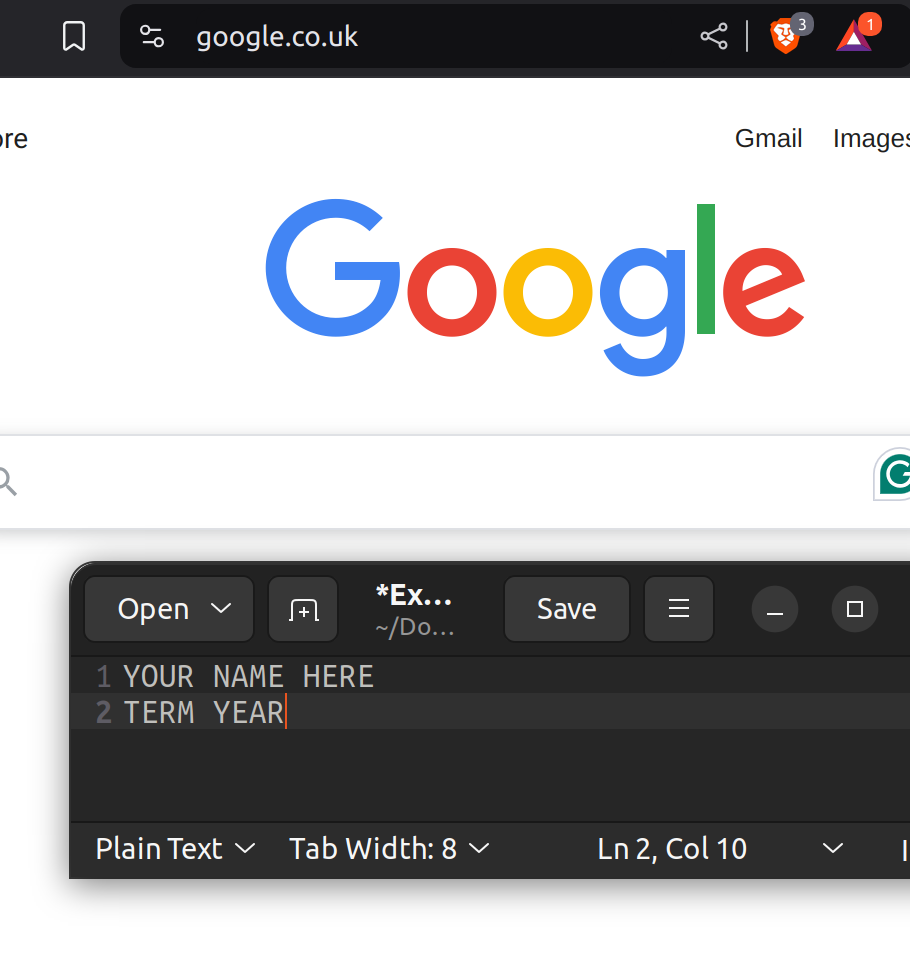
\includegraphics[scale=.2]{ExampleScreenshot.png}}
    \caption{This is an image of what each of your screenshots should look like}
    \alt{Example screenshot: a web browser showing the Google home page, with a small text editor window in front of it that says YOUR NAME HERE and TERM YEAR}
\end{figure}

\subsection*{Set up VirtualBox}
\begin{enumerate}
    \item Download and install VirtualBox, or another virtual machine program you prefer.
\end{enumerate}

\subsection*{Install Linux Mint}
\begin{enumerate}[start=2]
    \item Download Linux Mint. Any desktop edition is fine.
    \item In VirtualBox, create a new virtual machine and use the Mint download to start it.
    \item When Mint starts, double click the Install Linux Mint icon and follow the steps. The Linux Mint installation guide can help if you get stuck.
    \item You'll make a username and password during the install. Don't lose them! If you do, you'll need to reinstall the whole virtual machine.
\end{enumerate}

\subsection*{Install Kali Linux}
Choose one of these two ways to set up Kali:
\begin{enumerate}[start=6]
    \item \textbf{Easier:} download Kali's ready-made VirtualBox image, and import it by following Kali's guide. The default username and password are both \texttt{kali}. Change the password after you log in.
    \item \textbf{Full install:} download the Kali installer, and follow Kali's guide to installing it in VirtualBox. You'll create your own username and password during the install.
\end{enumerate}
If the full install shows an error about the network mirror, continue without it. After the install finishes, follow Kali's guide to setting up its package repositories.

Kali no longer uses the root account by default, so log in with your own user. When a command needs admin rights, put \texttt{sudo} in front of it.

\subsection*{Check your settings}
\begin{enumerate}[start=8]
    \item Once each install is finished, open the virtual machine's Settings in VirtualBox, and go to Storage. Make sure the installer file (the ISO) has been removed, so the virtual machine starts from its own virtual hard disk. If you imported Kali's ready-made image, there's no ISO to remove.
\end{enumerate}

\section*{Deliverables}
One file that includes these 6 screenshots, clearly labelled. Individual image files aren't accepted, and each screenshot should show what's asked for, not your whole monitor.
\begin{enumerate}
    \item Mint, logged in
    \item Kali, logged in as your user
    \item A terminal open in Mint
    \item A terminal open in Kali
    \item The Storage settings for your Mint virtual machine
    \item The Storage settings for your Kali virtual machine
\end{enumerate}

\section*{Resources}
References, a video, a PowerPoint and some notes are available at my website
Link: \href{https://www.aholdengouveia.name/InfoSec/InfoSecWk1.html}{\textbf{\nolinkurl{https://www.aholdengouveia.name/InfoSec/InfoSecWk1.html}}}

VirtualBox downloads
Link: \href{https://www.virtualbox.org/wiki/Downloads}{\textbf{\nolinkurl{https://www.virtualbox.org/wiki/Downloads}}}

Linux Mint download
Link: \href{https://www.linuxmint.com/download.php}{\textbf{\nolinkurl{https://www.linuxmint.com/download.php}}}

Linux Mint installation guide
Link: \href{https://linuxmint-installation-guide.readthedocs.io/en/latest/}{\textbf{\nolinkurl{https://linuxmint-installation-guide.readthedocs.io/en/latest/}}}

Kali Linux downloads, including the ready-made virtual machine images
Link: \href{https://www.kali.org/get-kali/}{\textbf{\nolinkurl{https://www.kali.org/get-kali/}}}

Kali guide: importing the ready-made VirtualBox image
Link: \href{https://www.kali.org/docs/virtualization/import-premade-virtualbox/}{\textbf{\nolinkurl{https://www.kali.org/docs/virtualization/import-premade-virtualbox/}}}

Kali guide: installing Kali in VirtualBox
Link: \href{https://www.kali.org/docs/virtualization/install-virtualbox-guest-vm/}{\textbf{\nolinkurl{https://www.kali.org/docs/virtualization/install-virtualbox-guest-vm/}}}

Kali guide: setting up the package repositories
Link: \href{https://www.kali.org/docs/general-use/kali-apt-sources/}{\textbf{\nolinkurl{https://www.kali.org/docs/general-use/kali-apt-sources/}}}

UTM, for Apple Silicon Macs
Link: \href{https://mac.getutm.app/}{\textbf{\nolinkurl{https://mac.getutm.app/}}}

\end{document}